\documentclass[math]{cours}
\author{Jean-Louis Halpérin}
\title{Introduction au Droit Public Français}
\date{2024-2025}
\begin{document}
\bettertitle

\section*{Informations}
Site du cours: \url{www.droit.ens.fr}\\
Chaque semaine, préparer un exposé sur l'arrêt (3mn au début) pour progresser. 2h de cours + 1h de review de décisions de justice.\\
Adresse: \url{mailto:jean-louis.halperin@ens.fr}

\section{L'Ordre Judiciaire}
\subsection{Les règles de droit}
	Définition essentialistes du droit et définition formalistes: Le droit est avant tout une technologie, définition dite positiviste.
	On définit une règle de droit comme ce qui est reconnu par une juridiction, par un jury.
	Hermann Kantovitch appelle ceci le critère de justiciabilité: la règle de droit, c'est ce qui est reconnu par des juges.
	On répond à cela que s'intéresser aux décisions judiciaires c'est s'intéresser à la pathologie du droit.
	Heureusement, il n'y a pas que des situations qui sont contestées.
	Il y a toutes formes de situations juridiques qui se déroulent sans procès.
	De même que les médecins apprennent l'anatomie au travers des maladies, on apprend le droit à travers ses problèmes. \\

	En France il y a deux ordres juridictionnels:
	\begin{enumerate}
		\item L'ordre judiciaire (civil et pénal), juridiction judiciaire, juge judiciaire. Au sommet: la cour de cassation.
		\item L'ordre administratif, avec les juridictions administratives. Au sommet: le conseil d'état.
	\end{enumerate}
	Au dessus de ceci se situe le \emph{Tribunal des Conflits}, qui arbitre lorsqu'il y a un conflit et qu'on ne sait pas quelle juridiction doit la décider.
	Il ne s'agit pas d'une cour suprême qui décide notre droit.
	Le Conseil Constitutionnel n'est pas une cour constitutionnelle, il ne rend que des décisions, et si elles ont beaucoup d'influence, il ne peut pas casser un arrêt de la cour de cassation ou du conseil d'état.
	Ce n'est par exemple pas le cas en Allemagne.
	Le Conseil Consitutionnel est en dehors de l'organisation juridictionnelle, même s'il entretient des rapports forts avec celle-ci.

	Il y a une hiérarchie au sein des ordres juridictionnels, les \emph{cours} se situent au dessus des \emph{tribunaux}.
	Les tribunaux rendent des \emph{jugements} et les cours rendent des \emph{arrêts}.
	On peut parler de \emph{décision} judiciaire pour tout tribunal sans être propre, mais c'est le terme technique (et le seul donc) qui peut être employé pour le Conseil Constitutionnel.
	Attention: en droit, tout est arbitraire et décidé par un législateur. \\

	Les cours peuvent être classées en différentes juridictions (civile et pénale ou répressive).
	La distinction se fait notamment sur les parties au procès:
	\begin{description}
		\item[Au Civil] Il y a au moins deux personnes (privées).
		\item[Au Pénal] Il oppose toujours l'état (représenté par le ministère public) à une personne qui est \emph{oursuivie}.
	\end{description}
	Le procès administratif a en général lieu entre une personne et un acte, et non contre un fonctionnaire ou l'état comme personne morale.
	Les juridictions pénales jugent les causes qui relèvent du droit pénal, qui sont en grande partie (mais pas en totalité) énuméré dans le code pénal (code Badinter qui a remplacé le code Napoléonien).
	Il y a des lois en dehors du code, par exemple la loi sur la presse.
	Les règles pénales répriment ce qu'on appelle des infractions.
	Les infractions sont divisées en trois niveaux:
	\begin{enumerate}
		\item Les contraventions (de police) qui ne peuvent être punies que d'une peine d'amende
		\item Les délits qui peuvent être punis d'amendes plus lourdes et d'emprisonnement jusqu'à 10 ans
		\item Les crimes qui sont punissables, outre des amendes, de réclusion criminelle entre 15, 20, 30 ans et perpétuité.
	\end{enumerate}
	Les peines présentées dans le code pénal sont les peines maximales, que le juge ne peut pas dépasser.
	Il n'y a pas lieu de s'étonner sur le fait que les peines ne soient pas toujours maximales, en vertu de l'individualisation du droit.
	Le terme délit est un des termes les plus équivoques qui soient:
	\begin{enumerate}
		\item Infractions jugées par le tribunal correctionel, niveau entre les contraventions et les crimes
		\item En droit pénal, peut désigner l'ensemble des infractions
		\item En matière de responsabilité civile (pour obtenir des dommages et intérêts), on parle de \emph{délit civil}.
	\end{enumerate}
	Le terme d'\emph{infraction} qui vient du verbe latin \emph{infringere} (on dit que les contrevenants à la loi, violent la loi).
	Cette expression est impropre.
	Par exemple, s'agissant du vol, le voleur ne viole pas les règles du code pénal, puisque celui-ci n'interdit pas de voler, mais à partir du moment où il est poursuivi, déclenche l'application des règles du code pénal.
	Les voleurs ne violent pas la loi, mais en déclenchent l'application.
	Dans la définition du procès pénal, les magistrats du ministère public (partie des magistrats: procureur, vice-procureur, substitut du procureur), souvent qualifié de magistrats du \emph{parquet}, ont le quasi-monopole de la poursuite.
	Quasi-monopole car certaines administrations (ponts et chaussées, eaux et forêts, bois\ldots) ont dans leurs attributions la capacité de donner des contraventions.
	Le parquet agit principalement sur des informations fournies par des personnes qui dénoncent des infractions ou s'en plaignent.
	La \emph{dénonciation} est l'acte d'informer le procureur de la République de la connaissance d'une infraction que l'on juge devoir être punie.
	La dénonciation n'est pas une \emph{délation}, et est même quelque chose d'honorable.
	Elle peut être faite par la victime elle-même (qui a plutôt intérêt à porter plainte) ou par n'importe quel tiers.
	Il n'y a pas d'obligation de dénonciation, sauf pour les autorités constituées, c'est à dire les fonctionnaires publics cf Article 40 du code de procédure pénale.
	Les fonctionnaires ont l'obligation de dénoncer ce qu'ils voient dans \textbf{l'exercice de leurs fonctions}.
	Une interprétation toutefois peut dire qu'une accusation ne peut pas se faire par ouï-dire.
	Certaines autres interprétations disent qu'il faut repasser par le chef d'établissement et d'autres qu'il ne faut agir qu'en considération de la victime.
	C'est une obligation qui n'est pas sanctionnée pénalement, et qui est rarement (presque jamais) sanctionnée disciplinairement.
	Ce n'est pas le seul cas d'une obligation non sanctionnée.\\

	L'audition d'une dénonciation se fait en commissariat ou en gendarmerie et peut donner lieu à une main courante ou à une plainte (appelée plainte simple).
	Le ministère public a le pouvoir de trancher sur l'opportunité des poursuite:
	pour toutes les dénonciations et plaintes, le ministère public a la possibilité de les classer sans suite,
	ou parce que le fait délictueux (au sens général) est mal établi, que le fait ne constitue pas une infraction,
	que le ministère public juge qu'il n'est pas bonne politique de poursuivre ce genre de fait.
	Il est possible de vaincre le classement sans suite en portant plainte avec constitution de partie civile:
	la constitution de partie civile peut avoir lieu à n'importe quel moment dans la procédure pour réclamer des dommages et intérêts.
	La victime a le choix soit d'aller au civil en parallèle de la procédure pénale soit de se constituer partie civile.
	En début de procédure, la plainte avec constitution de partie civile oblige un juge d'instruction à lancer une instruction et force le ministère public à agir.
	Toute constitution de partie civile est accompagnée d'une consignation d'une somme d'argent qui vise à informer la personne qui se constitue partie civile de la gravité de la procédure, et en cas de relaxe ou d'acquittement, à qualifier la dénonciation de calomnieuse.
	Sur ces bases, le ministère public lance l'enquête via la police judiciaire.
	Il y a deux types d'enquêtes en France:
	\begin{enumerate}
		\item Enquête de \emph{flagrant délit}: quand le délit vient de se commettre et qu'il y a des témoins/des preuves.
			La police peut alors perquisitionner sans l'accord de la personne perquisitionnée entre 6h et 21h.
		\item Enquête \emph{préliminaire}: quand la police est informée par des dénonciations, plaintes ou son travail de surveillance et qu'elle repère quelque chose.
			Les pouvoirs des policiers sont plus faibles.
			Les perquisitions doivent notamment être autorisées par la personne.
	\end{enumerate}
	Depuis l'extrême fin du 20$^{e}$ siècle, il y a nombre de procédures alternatives pour éviter les tribunaux:
	\begin{itemize}
		\item Classement sans suite
		\item Prononciation d'une amende forfaitaire: pas de procès, constatation dans le procès-verbal par l'officier de police judiciaire.
			Si la personne accepte de payer, le montant est fixé entre 11 et 3000€.
			Sinon, ce qui arrive en moyenne 10 millions de fois par an, on entre dans le cas de l'amende forfaitaire majorée.
		\item L'ordonnance pénale (depuis 1999, utilisée surtout pour les délits routiers et les stupéfiants):
			le ministère public établit la sanction pour les contraventions ou pour des délits mineurs,
			la personne est informée mais ne sera pas convoquée, le juge du tribunal de police (ou correctionnel) appose simplement sa signature
		\item La composition pénale :
			sur proposition du ministère public, non nécessairement l'amende maximale mais non nécessairement.
			La personne est convoquée et si elle ne s'y rend pas, le juge du tribunal de police (ou correctionnel) approuve la peine proposée par le ministère public.
		\item La Comparution Avec Reconnaissance Préalable de Culpabilité:
			la personne est convoquée et peut faire valoir son argument (souvent avec son avocat),
			le ministère public propose une peine inférieure à celle maximale en échange de la reconnaissance de culpabilité.
			Le président du tribunal correctionnel habilite la procédure.

		\item Le cas le plus classique:
			à l'issue d'une enquête de PJ, on prévient la personne visée (le prévenu) et il y a un procès.
		\item La comparution immédiate (flagrant délit):
			Enquête très rapide et comparution dans les quelques jours.
			La personne peut refusée d'être jugée si rapidement.
			Il n'y a pas de décision de comparution immédiate sans l'accord (un peu contraint) de la personne prévenue.
	\end{itemize}
	Les statistiques judiciaires sont sous forme d'une brochure qui donne les chiffres de 2 ans auparavant appelées \textit{Les chiffres-clefs de la justice}.
	Il y a aussi un petit peu de propagange appelée \textit{La Réponse Pénale}.
	Le non-lieu, l'absence de jugement et le classement sans suite sont considérées comme des réponses pénales.
	En 2022: il y a 648889 décisions pénales, 83\% des tribunaux correctionnels, 5\% des tribunaux de police pour 1800000 décisions civiles.\\

	Il y a 8800 magistrats en France. La loi Dupont-Moretti prévoit une augmentation du nombre de postes.
	Les magistrats sont des fonctionnaires dont le statut particulier est régi par une ordonnance de 1958.
	Il y a un seul statut, un seul corps, mais des positions diverses dans la carrière:
	ou bien dans le siège ou bien dans le parquet.
	La plupart des magistrats alternent dans leur carrière, mais ne peuvent occuper les deux à la fois.
	Les magistrats dépendent du Conseil Supérieur de la Magistrature, dernièrement révisé en 2008 (application en 2011).
	Le CSM n'est plus présidé par le Président de la République.
	Il est composé de deux formations, une pour ceux du siège et une pour ceux du ministère public.\\

	La formation compétente pour les magistrats du siège comporte 7 magistrats, le Premier, 6 magistrats élus, un conseiller d'état élu par ses pairs, un avocat élu par le Conseil national du barreau, et 6 personnalités qualifiées nommées.
	Concernant la formation des magistrats, le CSM fait une proposition au Président de la République.
	Le CSM choisi les magistrats supérieurs (par ancienneté dans la carrière souvent).
	Pour les autres magistrats, le ministère de la justice fait une proposition, et le CSM doit l'accepter par ce qu'on appelle un \emph{avis conforme}.
	Un avis peut être \emph{simple} que l'autorité qui demande l'avis n'est pas tenue de suivre, ou \emph{conforme} auquel cas l'autorité concernée par l'avis est tenue de suivre.
	C'est aussi cette formation qui est compétente pour juger les magistrats du siège selon les manquements dans leurs fonctions.
	Le ministère est tenu de suivre cet avis.\\
	La formation du parquet comporte 5 magistrats du parquet, un du siège et les 8 mêmes non-magistrats que celle du siège.
	En matière de nomination, le CSM fait des propositions que le président de la république n'est pas juridiquement tenu de suivre.
	En matière disciplinaire, la formation des magistrats du parquet rend un avis que le ministère n'est pas tenu de suivre.

\subsection{Formation des Tribunaux}
	Les Lois Taubira, Belloubet et LOPJ (loi Dupont-Moretti) ont réformé le système de tribunaux français.
	La loi Belloubet de 2019 a fusionné les Tribunaux de Grande Instance (TGI) et Tribunaux d'Instance.
	On parle maintenant de Tribunaux Judiciaires (TJ). Il y en a 164 dans les villes où siégaient un TGI et TI.
	Il y en a au moins un par département.
	Le TJ est, en matière civile, la juridiction de droit commun (qui règle le plus grand nombre d'affaires).
	D'abord pour les affaires personnelles et mobilières au dessus de 10000€, l'état des personnes (mariage, PACS, naissance, nationalité), la propriété immobilière, les brevets, les grèves\ldots
	Les TJ ont rendu 1,4 millions de décisions en 2022.
	Ils siègent en général à 1 ou 3 juges, mais il y a de plus en plus de procédures à 1 juge ou sans audience.
	Le président est juge des référés (référé civil, procédure d'urgence qui ne va pas rentrer dans les détails de l'affaire, qui va accorder une provision, interdire une publication.). Il y a eu 105000 décisions en référé en 2022.
\begin{figure}[h]
	\centering
	\begin{tikzpicture}
		\node{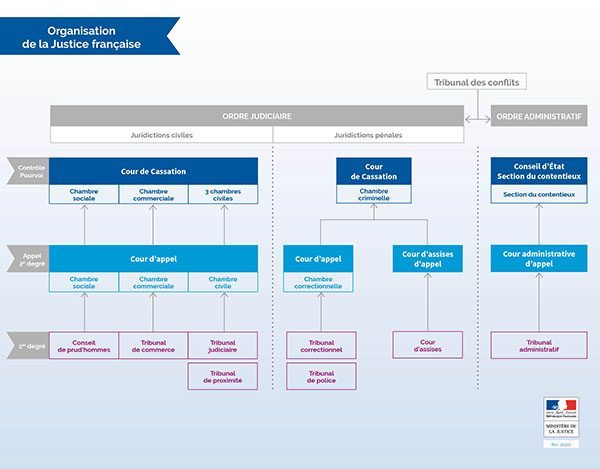
\includegraphics{orga_juridictionnelle}};
	\end{tikzpicture}
	\caption{L'organisation juridictionnelle}
	\label{fig:orga_juridictionnelle}
\end{figure}
	Dans 125 villes françaises qui avaient un TI mais pas de TGI, ont été maintenus des Tribunaux de Proximité (TP).
	Des juges du contentieux de la protection (JCP) y décident des affaires de surendettement, de crédit à la consommation, de bail d'habitation, de protection des majeurs, d'explulsion.
	Les JCP jugent à juge unique.\\
	Les contraventions des 5 classes sont jugées par les tribunaux de police (53000 jugements pour les 4 premières classes), auxquelles s'ajoutent les décisions d'ordonnance pénale.
	Les tribunaux correctionnels jugent les délits (avec des peines d'amende >3500€ et/ou de l'emprisonnement jusqu'à 10 ans).
	Depuis 2020, les peines de prison de moins d'un mois ne peuvent plus être prononcées\footnote{Il y a 85000 personnes dans les prisons françaises, pour 59000 places. La justice pénale française n'est donc pas laxiste.}.
	Les TCs peuvent produire des sanctions alternatives (bracelet électronique, travaux d'intérêt généraux\ldots). Ils rendent 580000 décisions par an.\\
	Toujours rattachés aux TJ, les juges d'instruction instruisent les crimes et les délits complexes (cumul d'infraction, délit nécessitant une instruction permettant de poursuivre l'enquête par une mise en examen).
	Depuis 2000 et la loi sur la présomption d'innocence, le juge d'instruction ne peut plus procéder à une décision de détention provisoire, et doit alors décider avec le juge des libertés et de la détention provisoire.
	C'est en principe une exception en cas de risque pour l'ordre public, les biens ou les personnes.\\
	Les juges des enfants siègent seuls ou dans l'un des 155 tribunaux pour enfants (avec 2 assesseurs non-professionnels).
	Le régime de traitement des mineurs est spécifique et existe depuis 1810 dans le code pénal ainsi que dans d'autres textes.
	Il existe également deopuis 2021 un code de la justice pénale des mineurs.
	Il a clarifié la question de la responsabilité ou de l'irresponsabilité pénale des mineurs.
	Il y a une distinction fondamentale qui est faite entre les mineurs discernents ou non-discernents.
	Être discernent c'est avoir conscience du fait de commettre un acte grave et d'avoir conscience de la sanction.
	Le code de 2021 établit la présomption qu'il n'y a pas de discernement du mineur avant 13 ans.
	À ce titre, les mineurs de moins de 13 ans sont présumés non-discernents et donc exempts de responsabilités.
	Au contraire, les mineurs de 13 à 18 ans sont présumés discernents.
	En chambre du conseil (à huis clos), pour les contraventions de 5ème classe et certains délits, le juge des enfants peut prononcer à l'égard des mineurs à partir de 10 ans et jusqu'à 13 ans des sanctions dites éducatives.
	Le mineur, s'il n'est pas en danger reste de sa famille, mais peut aussi être retiré à sa famille et placé en famille d'accueil, sous la tutelle de l'état ou dans un centre spécialisé.
	À partir de 13 ans, les mineurs peuvent être envoyés en prison, dans des centres éducatifs fermés, le code pénal prévoit des peines pour les mineurs réduites de moitié.
	Il y a des exceptions, notamment pour les grands mineurs (16-18 ans) récidivistes.
	Pour les crimes des mineurs entre 16 et 18 ans, la cour d'assises des mineurs. \\
	Il y a 134 tribunaux de commerce qui jugent les conflits entre commerçants (personne publiques inscrites au registre du commerce) ou des sociétés relatifs à des actes de commerce (\textit{faillite}, mot qui n'a plus de sens depuis les années 60).
	Les juges sont élus pour 4 ans par les commerçants et ont rendus 109000 décisions en 2022.\\
	Les conseils de prud'hommes (211 au lieu de 271 avant 2008) jugent les litiges individuels du travail.
	Les juges sont désignés en 5 sections (industrie, commerce, culture, professions libérales, cadres\ldots) siègent de manière paritaire en bureau de conciliation (au moins 2) ou de jugement (au moins 4).
	Ils comptent autant de représentant des employés que des patrons.
	Ils ont rendu 113000 décisions en 2022.\\
	Les 272 tribunaux paritaires des baux ruraux règlent les conflits sur les baux ruraux sont des juridictions avec des juges élus par les représentants syndicaux des propriétaires et locataires de baux et sont placés sous la présidence d'un juge professionnel.
	On appelle ce type de juridiction avec des professionnels et non-professionnels des juridictions \emph{d'échevinage}.\\
	La cour d'assises (avec la cour criminelle départementale) sont composées (en première instance) de 3 magistrats professionnels et de 6 jurés (9 en appel) tirés au sort.
	Il y en a une par département, c'est une formation temporaire (qui juge par session).
	Les cours d'assises jugent de crimes (réclusion de 15 ans à perpétuité).
	Les personnes traduites devant une cours d'assises s'appellent \emph{accusées} et non prévenues.
	Magistrats et jurés délibèrent ensemble et sur la culpabilité et sur la peine.
	Les cours départementale criminelles (ou tribunaux criminels) devant lesquelles sont jugés les crimes passibles de réclusion criminelle de 15 et 20 ans (par exemple les viols).
	Les tribunaux criminels n'ont pas de jury et sont composés de 5 magistrats, mais suivent la même procédure.
	Les peines criminelles peuvent être accompagnées d'une peine incompressible de sûreté durant laquelle aucune réduction ni libération ne peut avoir lieu.
	En dehors de cette période, les réductions sont courantes et sont appliquées par le Juge d'Application des Peines (JAP).
	La perpétuité réelle existe tout de même, même si on la voit peu.\\
	Les cours d'appel sont séparées en de multiples chambres (civiles (appels des TJ mais peu des JCP), commerciales (appels des tribunaux commerciaux), sociales (appels des prud'hommes) et de l'instruction (appels des décisions prises par les juges d'instructions ou les juges des libertés et la détention)).
	Le délai d'appel est de 10 jours au pénal, 1 mois au civil.
	La décision peut être mise en suspens pendant la procédure d'appel.\\
	La cour de cassation (créée le 27 novembre 1990, sujet de la thèse de JLH) est composée d'une centaine de magistrats, composées de 6 chambres (3 civiles, une sociale, une pénale, une commerciale).
	Dans chaque chambre siègent un nombre de conseillers à la cour de cassation.
	Chaque chambre à un président et à la tête de la cour un premier président (appelée le Premier).
	Il y a un parquet auprès de la cour de cassation composé du procureur général de la cour de cassation, d'avocats généraux (ce ne sont pas des avocats mais les assistants aux procureurs généraux).
	Le pourvoi (ou recours) en cassation (procédure intentée par une partie qui a perdu en cour d'appel, qui n'est pas un troisième degré de justice),
	demande à la cour de cassation de ne pas se prononcer sur le fond de l'affaire mais sur le respect du droit par la cour d'appel.
	La cour de cassation est très sollicitée (15000 décisions au civil, 7000 au pénal).
	Par comparaison, le conseil d'état juge (9000 affaires par an).
	Depuis 2002, il y a une procédure de non-admission qui permet de rejeter les pourvois non sérieux.
	Tout pourvoi doit être soutenu par un avocat.
	Depuis 1970, pour juger des affaires plus sérieuses, on convoque l'assemblée plénière (19 membres: Premier, présidents, doyens, membres des chambres).
	Au cas où après un pourvoi en cassation et un renvoi en cour d'appel, il y a un deuxième pourvoi, ou bien il y a rejet, ou bien l'assemblée plénière juge.
	Il n'y a pas d'effet suspensif au civil mais au pénal si, ce qui a été très important avant l'abolition de la peine de mort.
	Il y a ouverture à cassation en cas de:
	\begin{itemize}
		\item violation de la loi en cour d'appel,
		\item violation des formes de procédure,
		\item défaut de base légale,
		\item excès de pouvoir
	\end{itemize}
	Toutes les décisions de justice doivent être motivés. La cour de cassation a imposé jusqu'à 2019 le style classique et laconique des décisions.
	La motivation d'une décision de justice se présente sous une phrase commençant par \textit{Attendu que} et comportant de nombreuses subordonnant.
	Elle doit contenir un visa, i.e. l'évocation d'un texte de loi.
	On utilise désormais un style plus direct pour les attendus. \\
	En France, la jurisprudence désigne les décisions judiciaires qui tranchent un procès et posent une norme individuelle (qui ne concerne que les parties au procès) et qui vont d'une certaine manière servir de précédent, être imitées, reprises et être transformées en une norme globale.
	Les tribunaux créent du droit par la jurisprudence.
	Tous les énoncés de droit demandent à être interprétés et appliqués, et la norme est donc créée par l'interprétation et donc par la décision judiciaire.
	L'article 5 du code civil (inchangé depuis 1804) interdit à toute juridiction de créer des arrêts de réglement.
	Le même code civil dit dans l'article 4 que le juge qui ne tranche pas un procès commet une faute grave.
	Le juge ne peut pas s'abriter pour éviter de trancher sur le silence ou l'obscurité.
	C'est le juge qui dit si un texte est clair ou non, et notamment les juges suprêmes. Ce sont eux qui posent la norme, mais pourquoi ?
	Notamment de par une loi de 1837 qui a inauguré le mécanisme de l'assemblée plénière qui force la cour d'appel à suivre la décision de l'assemblée plénière.
	Certains disent que le législateur laisse aussi faire, parce que les parlementaires n'y connaissent rien.
	Ainsi, certaines normes individuelles sont transformées en normes générales.

\subsection{Etude d'une décision de la 1ere Civ du 9 Oct 2001}
	Voir \url{https://www.courdecassation.fr/decision/export/60794d029ba5988459c47cc3/1}\\
	M. Franck X a perdu devant la cour d'appel.
	La naissance a eu lieu en 76, la décision en 2001. Il n'y avait pas prescription, celle-ci étant suspendue pendant la minorité de l'enfant.
	La cour de cassation n'a pas obligation de répondre à tous les moyens (subdivision de l'argumentation pour ne pas mêler les reproches à la cour d'appel), même si elle l'a fait ici.
	Ici, on a une affaire civile car il s'agit d'une clinique privée, sinon, il s'agirait d'une affaire renvoyée devant le tribunal administratif à l'origine.
	La cour de cassation considère ici qu'il y a eu un vice de procédure.
	La cour de cassation considère que le médecin n'a pas rempli son contrat et casse donc la décision, la renvoyant devant la cour d'appel de Grenoble.
	Dans les années 70 (après 1975), s'est développé une jurisprudence demandant aux médecins de donner aux patients le maximum d'informations, notamment sur les risques encourus.
	Le patient ou son représentant signe alors un document précisant qu'il est bien informé.
	L'information par le médecin s'étend à des cas imprévus en cas d'opération et ne s'applique pas en état d'urgence.
	Le médecin doit continuer à informer la femme pendant l'accouchement.
	Le médecin s'est défendu en disant qu'il n'avait pas manqué à une obligation qui n'existait pas encore.\\

	Ici, le premier paragraphe explique la situation causant litige.
	Les deux suivants résument la conclusion de l'appel.
	Le dernier donne la réponse de la cour de cassation (\textit{cependant}) et son arrêt.
	La cour de cassation voit, au milieu de l'accouchement, que le médecin viole le principe constitutionnel de sauvegarde de la dignité humaine.
	Ce principe n'est pas clairement écrit dans la constitution, mais est lu entre les lignes du préambule de la constitution de 1958 qui fait référence à celui de la constitution de 1946 qui parle de la victoire contre les puissances qui ont voulu asservir l'homme.
	La jurisprudence de l'époque précisait que le médecin était dans son droit, mais la cour de cassation juge que l'interprétation jurisprudentielle ne doit pas dépendre de la période ou les faits se sont produits.
	Il faut appliquer rétroactivement une règle nouvelle qui était imparfaitement connue au moment des faits.
	\textit{Nul ne doit se prévaloir d'un droit acquis à une jurisprudence figée}, il est tout à fait possible pour la cour de cassation de changer la jurisprudence,
	et le plaideur ne peut se plaindre de la différence de jugement rendu entre deux époques différentes.

\section{Le cours d'après}

\subsection{Etudes de Décisions}
\subsubsection{Chambre Criminelle 25 Février 2014}
Décision trouvable à \url{https://www.legifrance.gouv.fr/juri/id/JURITEXT000028669325}

Dans cette décision, la cour de cassation étudie le pourvoi de Mme Y contre la cour d'appel de Paris.
La cour d'appel avait déboutée Mme Y de sa plainte en diffamation publique en exposant dans son arrêt que:
\begin{itemize}
	\item Donner une image peu reluisante (termes \textit{fêtarde}, \textit{adepte de la chouille}) n'est pas contraire à la dignité humaine et ne caractérise pas une diffamation.
	\item Qu'utiliser des termes triviaux en les incluant dans un propos ne constitue pas un comportement déshonorant et ne caractérise pas une injure.
\end{itemize}
Sur ces deux moyens, la cour de cassation va pointer des contradictions de la cour d'appel:
\begin{itemize}
	\item Donner des faits précis pouvant porter atteinte à l'honneur et à la considération caractérise le délit de diffamation publique.
	\item Le contexte d'un article de presse, même si le propos lui-même peut ne pas revêtir, dans un cercle privé, le caractère d'injure, constitue une injure et caractérise une injure publique
\end{itemize}
C'est pourquoi la cour de cassation va casser le jugement de la cour d'appel pour défaut de motifs et manque de base légale.

\subsubsection{Première Chambre Civile 14 Novembre 2006}
Décision trouvable sur \url{https://www.legifrance.gouv.fr/juri/id/JURITEXT000007055276}

L'affaire oppose l'association Croyances et libertés à la société GIP sur une parodie de la cène à des fins publicitaires
Dans cet arrêt, la 1ère Chambre Civile étudie deux pourvois:
\begin{enumerate}
	\item Le premier pourvoyé par GIP pour vice de procdéure et manque de de citation envers le directeur de GIP
	\item Le second pourvoyé par C\&L pour avoir déclaré recevable l'intervention de la LDH qui:
		\begin{enumerate}
			\item Par la loi du 29/07/1881, n'aurait pas dû pouvoir exercer des droits autres que ceux de la partie civile et n'aurait pas dû pouvoir défendre en justice un motif qui n'est pas celui qu'elle est habilitée à défendre (ici le respect de la DDHC).
			\item Que la cour d'appel autorisant cela a violé le code de procédure civile.
		\end{enumerate}
\end{enumerate}
À ceci, la cour de cassation répond que:
\begin{enumerate}
	\item L'avocat de la GIP ayant démontré dans ses réponses une parfaite connaissance du dossier n'a pas manqué de temps
	\item La cour d'appel:
		\begin{enumerate}
			\item a eu raison d'autorisé l'intervention de la LDH qui se basait sur la convention de sauvegarde des droits de l'homme et des libertés fondamentales
			\item a eu tort de retenir l'existence d'un trouble quand la seule parodie de la Cène est faite sur la forme de sa représentation et n'a pas pour but d'outrager.
		\end{enumerate}
\end{enumerate}
La cour de cassation rejette donc les deux pourvois, mais casse et annule la décision de la cour d'appel, à l'exception de la recevabilité de la LDH et confirme l'absence d'exception de nullité.
Toutefois, la Cour de cassation met fin au litige plutôt que de renvoyé et condamne C\&L aux dépens.

\subsection{}

\end{document}
